\section{SISO Pole Placement}
This section primarily holds for SISO systems but with some restrictions also for the MIMO case (see end of this section).
\subsection{Full State Feedback}
Assuming the internal state of a system can be accessed completely, the system can be controlled
with a \textit{reference signal} $r$ (scalar) \textit{scaling vector} $\mathbf{S}$ (column vector) and a static gain $\mathbf{K}$ (row vector):
\begin{center}
    % \includegraphics[width = \linewidth]{full_state.png}
    \usetikzlibrary{shapes,arrows,positioning,calc}

\tikzset{
    block/.style = {draw, fill=white, rectangle, minimum height=3em, minimum width=3em},
    tmp/.style  = {coordinate},
    sum/.style= {draw, fill=white, circle, node distance=1cm},
    input/.style = {coordinate},
    output/.style= {coordinate},
    pinstyle/.style = {pin edge={to-,thin,black}
        }
}


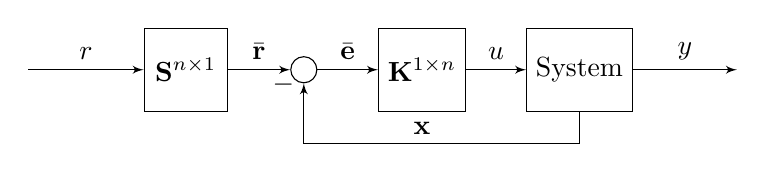
\begin{tikzpicture}[auto, node distance=2cm,>=latex']
    \node [input, name=rinput, node distance=1.5cm]         (rinput)        {};
    \node [block, right of=rinput]                          (scale_vec)     {$\mathbf{S}^{n\times 1}$};
    \node [sum, right of=scale_vec, node distance=1.5cm]    (sum1)          {};
    \node [block, right of=sum1, node distance=1.5cm]       (static_gain)   {$\mathbf{K}^{1\times n}$};
    \node [tmp, below = 0.4cm of static_gain]               (tmp1)          {$\mathbf{x}$};
    \node [block, right of=static_gain]                     (sys)           {System};
    % \node [output, below of=sys] (x) {};
    \node [output, right of=sys, node distance=2cm] (output) {};
    \node at (5,-.75) {$\mathbf{x}$} ;

    \draw [->] (rinput) -- node{$r$} (scale_vec);
    \draw [->] (scale_vec) -- node{$\bar{\mathbf{r}}$} (sum1);
    \draw [->] (sum1) -- node{$\bar{\mathbf{e}}$} (static_gain);
    \draw [->] (static_gain) -- node{$u$} (sys);
    \draw [->] (sys) -- node{$y$} (output);
    \draw [->] (sys) |-(tmp1) -| node[pos=0.99] {$-$} (sum1);
\end{tikzpicture}
\end{center}

The corresponding closed-loop system is
\noindent\begin{align*}
    \dot{\mathbf{x}} & =(\mathbf{A}-\mathbf{BK})\mathbf{x}+\mathbf{B}\bar{N}r, & \bar{N}=\mathbf{KS} \\
    y                & =(\mathbf{C}-\mathbf{DK})\mathbf{x} +\mathbf{D}\bar{N}r
\end{align*}
Remarks:
\begin{itemize}
    \item $(\mathbf{A}-\mathbf{BK})$ determines the closed-loop dynamics
    \item zeros are not affected by feedback
\end{itemize}

\subsection{Pole Placement}\label{sec:pole_placement}
Pole placement can be used to tune $\mathbf{K}$ and $\mathbf{S}$ to achieve the desired closed loop poles $\lambda_i$ of a controllable system.
The desired characteristic equation is
\noindent\begin{align*}
    \varphi_{cl,des} & =\det{(s\mathbf{I}-\mathbf{A}+\mathbf{BK})}=(s-\lambda_1)(s-\lambda_2)\ldots(s-\lambda_n) \\
                     & =s^n+\alpha_{n-1}s^{n-1}+\ldots+\alpha_0
\end{align*}

\subsubsection{Reachable Canonical Form}
If the system is in \textbf{reachable canonical form} and $\mathbf{K} = \left[k_0,k_1,\ldots,k_{n-1}\right]$, then

    {\footnotesize
        \noindent\begin{equation*}
            \mathbf{A}_{\mathrm{cl}}=\mathbf{A-BK}=\begin{bmatrix}
                0        & 1        & \ldots & 0                \\
                0        & 0        & \ldots & 0                \\
                \vdots   & \vdots   & \ddots & 1                \\
                -a_0-k_0 & -a_1-k_1 & \ldots & -a_{n-1}-k_{n-1}
            \end{bmatrix}
        \end{equation*}
    }

and the closed-loop characteristic polynomial can be used to choose the parameters $k_i$ based on the desired parameters $\alpha_i$:
\noindent\begin{align*}
    \varphi(s) & =s^n+(a_{n-1}+k_{n-1})s^{n-1}+\ldots+(a_0+k_0) \overset{!}{=} \varphi_{cl,des} \\
    k_i        & =\alpha_i-a_i,i=0,\ldots,n-1
\end{align*}

\subsubsection{General Case}
If the system is \textbf{controllable} but not in reachable canonical form, the following steps have to be applied
\begin{enumerate}
    \item Calculate $\mathbf{A}'$ by comparing the characteristic polynomial of $\mathbf{A}$ with the one of the parametric $\mathbf{A}'$ from~\ref{RCF}.
    \item Find transformation matrix $\mathbf{T}$ (using $\mathbf{A}'$ from 1.\ and the known form for $\mathbf{B}'$ to calculate $\mathbf{R}'$):
          \noindent\begin{align*}
              \mathbf{R}' & =\begin{bmatrix}
                                 \mathbf{B}' & \mathbf{A}'\mathbf{B}' & \ldots & {(\mathbf{A}')}^{n-1}\mathbf{B}'
                             \end{bmatrix} \\
                          & =\mathbf{TR}  =\begin{bmatrix}
                                               0      & 0        & \dots               & 1     \\
                                               \vdots &          & \ddots              &       \\
                                               0      & 1        & -a_{n-1}            & \dots \\
                                               1      & -a_{n-1} & a_{n-1}^2 - a_{n-2} & \dots \\
                                           \end{bmatrix}                                \\
              \mathbf{T}  & = \mathbf{R'R}^{-1}
          \end{align*}
          with $\mathbf{R}'$ the reachability matrix of the transformed system.
          \begin{itemize}
            \item $a_i$ are the coefficients of $\mathbf{A}'$
            \item Note that there are 2 different ways to calculate $\mathbf{R}'$ of which we use the first one as $\mathbf{T}$ is unknown in the beginning.
          \end{itemize}
    \item Similarity transform of $\mathbf{A,B,C,D}$ into reachable canonical form $\mathbf{A',B',C',D'}$
    \item Apply method for reachable canonical form
          \begin{equation*}
              \mathbf{K}^{\prime} =\left[\alpha_{0}-a_{0},\quad\alpha_{1}-a_{1},\quad\ldots,\quad\alpha_{n-1}-a_{n-1}\right]
          \end{equation*}
    \item Transform $\mathbf{K}'$ back to the original system:
          \noindent\begin{equation*}
              \mathbf{K}          = \mathbf{K'RR}^{-1}
          \end{equation*}
          which is possible if $\mathbf{R}$ is invertible (corresponds to controllability).
\end{enumerate}

\textbf{Remarks}:
\begin{itemize}
    \item $\mathbf{A'},\mathbf{A}$ share their eigenvalues, therefore a comparison of coefficients can be used.
\end{itemize}

\newpar{}
\ptitle{Reminder}\label{RCF}

The reachable canonical form is given by

\begin{equation*}
    G(s)=\frac{b_{n-1}s^{n-1}+b_{n-2}s^{n-2}+\cdots+b_0}{s^n+a_{n-1}s^{n-1}+\cdots+a_0}+d\\
\end{equation*}
and
\begin{align*}
    \mathbf{A}' & =\begin{bmatrix}
                       0      & 1    & 0 & 0      & \cdots & 0        \\
                       0      & 0    & 1 & 0      & \cdots & 0        \\
                       \vdots &      &   & \ddots &        & 1        \\
                       -a_0   & -a_1 &   & \cdots &        & -a_{n-1}
                   \end{bmatrix}, & \mathbf{B}' =\begin{bmatrix}
                                                     0      \\
                                                     0      \\
                                                     \vdots \\
                                                     1\end{bmatrix}                             \\
    \mathbf{C}' & =\begin{bmatrix}
                       b_0 & b_1 & \cdots & b_{n-1}
                   \end{bmatrix},                     & \mathbf{D}'                     =[d];
\end{align*}

\paragraph{Unreachable/Uncontrollable Modes}
Controllability (or reachability) is a \textbf{necessary and sufficient condition} for \textbf{arbitrary} pole placement.
Conversely, in an uncontrollable system in modal coordinates there will be at least one state
\begin{equation*}
    \dot{\tilde{x}}_i\quad=\quad\lambda_i\tilde{x}_i+\tilde{b}_i u
\end{equation*}
for which $b_i=0$.
\begin{itemize}
    \item Hence, no matter how we choose $\mathbf{K}$, the pole $\lambda_i$ will remain in it's original location.
    \item Note however, that this doesn't make a statement on stability:
          \begin{itemize}
              \item If the system is not stabilizable (see definition) this is an issue.
              \item If the system is stabilizable, the unreachable modes will remain in their locations and e.g.\ slow down the system dynamics but the overall system will still be stable.
          \end{itemize}
\end{itemize}

\subsubsection{Ackermann's Formula}
Assuming that the system is \textbf{controllable}, Ackermann's formula can be used to calculate $\mathbf{K}$ for \textbf{both} CT and DT systems:
\noindent\begin{align*}
    \mathbf{K}               & =\begin{bmatrix}
                                    0, & \ldots, & 0, & 1
                                \end{bmatrix}
    \mathbf{R}^{-1}\varphi_{cl}(\mathbf{A})                                                               \\
    \varphi_{cl,des}(s)          & =s^n+\alpha_{n-1}s^{n-1}+\ldots+\alpha_0=(s-\lambda_1)\ldots(s-\lambda_n)  \\
    \varphi_{cl,des}(\mathbf{A}) & =\mathbf{A}^n+\alpha_{n-1}\mathbf{A}^{n-1}+\ldots+\alpha_0 \mathbf{I}      \\
                             & = (\mathbf{A}-\lambda_1 \mathbf{I})\ldots(\mathbf{A}-\lambda_n \mathbf{I})
\end{align*}

\newpar{}
\ptitle{Remarks}

\begin{itemize}
    \item The formulas are the same for \textbf{DT} as for CT but of course the poles must be placed in the unit disk instead of the LHP.
    \item \textbf{MATLAB}: \texttt{place} or \texttt{acker} (place uses more stable algorithm)
\end{itemize}

\subsubsection{Reference Scaling}
% TODO: This assumes D = 0, right?
To ensure that the closed-loop systems follows unit steps with zero steady state error, the scaling vector $\mathbf{S}$ has to be chosen accordingly
\noindent\begin{align*}
    G_{yr}^{cl}(s) & = G_{y\leftarrow r}^{cl}(s) =\mathbf{C}{(s\mathbf{I}-\mathbf{A}+\mathbf{BK})}^{-1}\mathbf{B}\bar{N}r,                                                                          & \bar{N}=\mathbf{KS} \\
                   & G_{y\leftarrow r}^{cl}(0)  \overset{!}{=} 1                                                                                                                                                          \\
    \bar{N}        & =-{\left[\mathbf{C}{(\mathbf{A}-\mathbf{BK})}^{-1}\mathbf{B}\right]}^{-1}                                                                                                                            \\\\
    \bar{N}        & =\underbrace{\left[\mathbf{CA}^{-1}\mathbf{B}\right]}_{\text{DC ol.}}\cdot\underbrace{{\left[\mathbf{C}{(\mathbf{A}-\mathbf{BK})}^{-1}\mathbf{B}\right]}^{-1}}_{\text{DC cl.}}
\end{align*}
In other words, the scaling vector $\mathbf{S}$ has to be chosen such that $\mathbf{KS}=\bar{N}$.

\subsubsection{Pole Placement for MIMO Systems}
\begin{itemize}
    \item If the system is controllable from any one of the inputs, pole placement works even though we might not use the full potential of all the inputs
    \item In addition to the poles, the closed-loop eigenvectors (modal shapes) can be placed
\end{itemize}
